% PLOS Digital Health — Research Article (New Methods)
\documentclass{article}

\usepackage[numbers]{natbib}
\usepackage{booktabs}
\usepackage{tabularx}
\usepackage{graphicx}
\usepackage{ragged2e}
\usepackage[table,xcdraw]{xcolor}
\usepackage{hyperref}
\usepackage{amsmath}
\usepackage[margin=1in,footskip=0.25in]{geometry}
\usepackage{setspace}
  \doublespacing
\usepackage{lineno}
  \linenumbers
\renewcommand{\figurename}{Fig}
\renewcommand{\tablename}{Table}

\begin{document}

%% ————————————————————————————————
%% TITLE PAGE
%% ————————————————————————————————

\title{Large language models for self-administered conversational vignette assessment of provider competencies: A pilot and validation study in Vietnam with automated LLM-powered transcript classification}

\author{
  Benjamin Daniels$^{1,2,\ast}$,
  Wenjia(Stella) Zhang$^{1}$,
  Hoang Nguyen$^{3,4}$,
  David Duong$^{5,6}$ \\[6pt]
  \small $^{1}$ Harvard T.H.\ Chan School of Public Health, Boston, MA, USA \\
  \small $^{2}$ gui2de, Georgetown University, Washington, DC, USA \\
  \small $^{3}$ Partnership for Health Advancement in Vietnam (HAIVN), Hanoi, Vietnam \\
  \small $^{4}$ Beth Israel Deaconess Medical Center (BIDMC), Boston, MA, USA \\
  \small $^{5}$ Harvard Medical School, Boston, MA, USA \\
  \small $^{6}$ Brigham and Women's Hospital, Boston, MA, USA \\[4pt]
  \small $^{\ast}$ Corresponding author: bdaniels@fas.harvard.edu
}

\date{}
\maketitle
\thispagestyle{empty}

\noindent \textbf{Short title:} AI-based clinical vignette assessment: Pilot and validation study in Vietnam

\newpage

%% ————————————————————————————————
%% ABSTRACT
%% ————————————————————————————————

\begin{abstract}
\noindent We developed and validated a self-administered clinical vignette platform powered by a large language model (LLM), deployed through a SurveyCTO web survey, to measure primary health care provider competencies in Vietnam. In a pilot focus group, nine physicians rated LLM-simulated patient interactions as realistic (mean 3.78/5) and user-friendly. In the validation phase, 22 providers completed 132 vignette interactions across ten clinical scenarios in Vietnamese. Essential diagnostic checklist scores (human-coded from translated transcripts) correlated with expert clinician evaluations (Pearson's $\rho$ = 0.55--0.60). LLM-automated coding of checklist items from translated English transcripts correlated reasonably with human coding ($\rho$ = 0.53), and coding directly from Vietnamese transcripts performed comparably ($\rho$ = 0.51), suggesting that a separate translation step may not be necessary. The total cost of 132 chatbot interactions was under USD 2. LLM-driven conversational vignettes represent a low-cost and scalable method for assessing provider competencies in respondents' local language, eliminating the need for extensive enumeration staffs while preserving the open-ended format critical to vignette validity, and additionally introducing flexible feature extraction from transcripts using grading rubrics. The platform is open-source and designed for replication in other health system contexts.
\end{abstract}

\newpage

%% ————————————————————————————————
%% AUTHOR SUMMARY
%% ————————————————————————————————

\section*{Author summary}

Measuring the clinical skills of healthcare providers is essential for improving the quality of care, but current survey methods are expensive and require trained enumerators to travel to health facilities in person. We developed a new approach that uses large language models (LLMs) -- the technology behind tools like ChatGPT and Claude -- to simulate patients in realistic clinical conversations that healthcare providers can complete on their phones or laptops over the Internet in their own language. In Vietnam, we tested this tool with 31 physicians across ten clinical scenarios. Providers found the simulated patient conversations realistic and easy to use. We also tested whether LLMs could automatically score the conversations, which showed reasonable agreement with human scoring, and performed nearly as well when scoring directly from Vietnamese, without requiring a separate translation step. When we compared these results from our tool against holistic expert physician ratings of the same conversations, the scores agreed well, suggesting that automatic transcript grading based on rubrics produces meaningful measures of clinical skill. This tool costs less than two US dollars for over a hundred consultations and required no in-person surveyors, making it potentially transformative for routine, large-scale monitoring of healthcare quality in resource-limited settings. The platform and code are openly available for adaptation.

\newpage

%% ————————————————————————————————
%% INTRODUCTION
%% ————————————————————————————————

\section{Introduction}

Human resources for health represent the majority of total health expenditures in most countries, yet investments in primary health care education and training have not consistently translated into improved clinical competencies \citep{ranson2010priorities, rowe2018effectiveness, daniels2024medical, lilford2025policy}. Clinical vignettes -- open-ended roleplay interactions with standardized patients -- have emerged as a primary method for measuring provider competencies across health systems \citep{who2022global, das2005which, leonard2005use, andrews2021quality}. By eliciting each provider's unprompted approach to diagnosis and management of simulated cases, vignettes measure the best possible standard of care that providers are capable of delivering \citep{das2007money, daniels2024medical}. However, traditional vignette surveys require two trained enumerators per interaction, significant travel budgets, and in-person coordination, making them expensive to deploy at scale or repeat at frequent intervals \citep{andrews2021quality, das2023prices}. Digital multiple-choice formats undermine validity because unprompted elicitation of knowledge is the foundation of the method \citep{das2005which}.

Recent advances in large language models (LLMs) have created new possibilities for scalable clinical assessment. LLM-based virtual patients can simulate realistic patient-clinician dialogues and provide automated performance feedback \citep{cook2025virtual}, and a rapidly growing literature has explored their use in medical education \citep{zeng2025embracing}. However, most existing applications target medical student training in high-income settings, and few have been validated against established competency measures or deployed for health workforce assessment in low- and middle-income countries, where the need is greatest \citep{zhang2026scoping}. Automated scoring of clinical interactions using LLMs has shown promise but remains noisy, with studies reporting moderate agreement with human evaluators at best \citep{geathers2025benchmarking, kuling2026assessment}. A tool that combines LLM-based patient simulation with automated data extraction -- validated against expert clinical judgment -- could enable routine, low-cost competency measurement without in-person enumerators.

This study presents such a tool: a new method for self-administered and automatically coded clinical vignettes using LLMs. We developed an LLM-based chatbot interface \citep{geiecke2024conversations, surveycto2025llm} using web-based SurveyCTO survey software compatible with mobile phones (\textbf{Figure \ref{fig:chatbot}}). In Vietnam, we piloted and validated this platform with primary health care providers across ten clinical scenarios. The chatbot -- powered by OpenAI (gpt-4.1-nano) -- role-played clinical cases in Vietnamese via respondents' personal mobile devices at a cost of under USD 2 for 132 interactions. We also developed an automated data extraction pipeline using Anthropic's Claude language model (claude-haiku-4-5) to classify provider performance from the resulting transcripts. We report results from (1) a focus group of 9 providers assessing usability and realism, and (2) a validation sample of 22 providers (132 interactions) comparing human-coded, LLM-coded, expert-graded, and knowledge-test-based competency measures.

\begin{figure}[htbp]
  \centering
  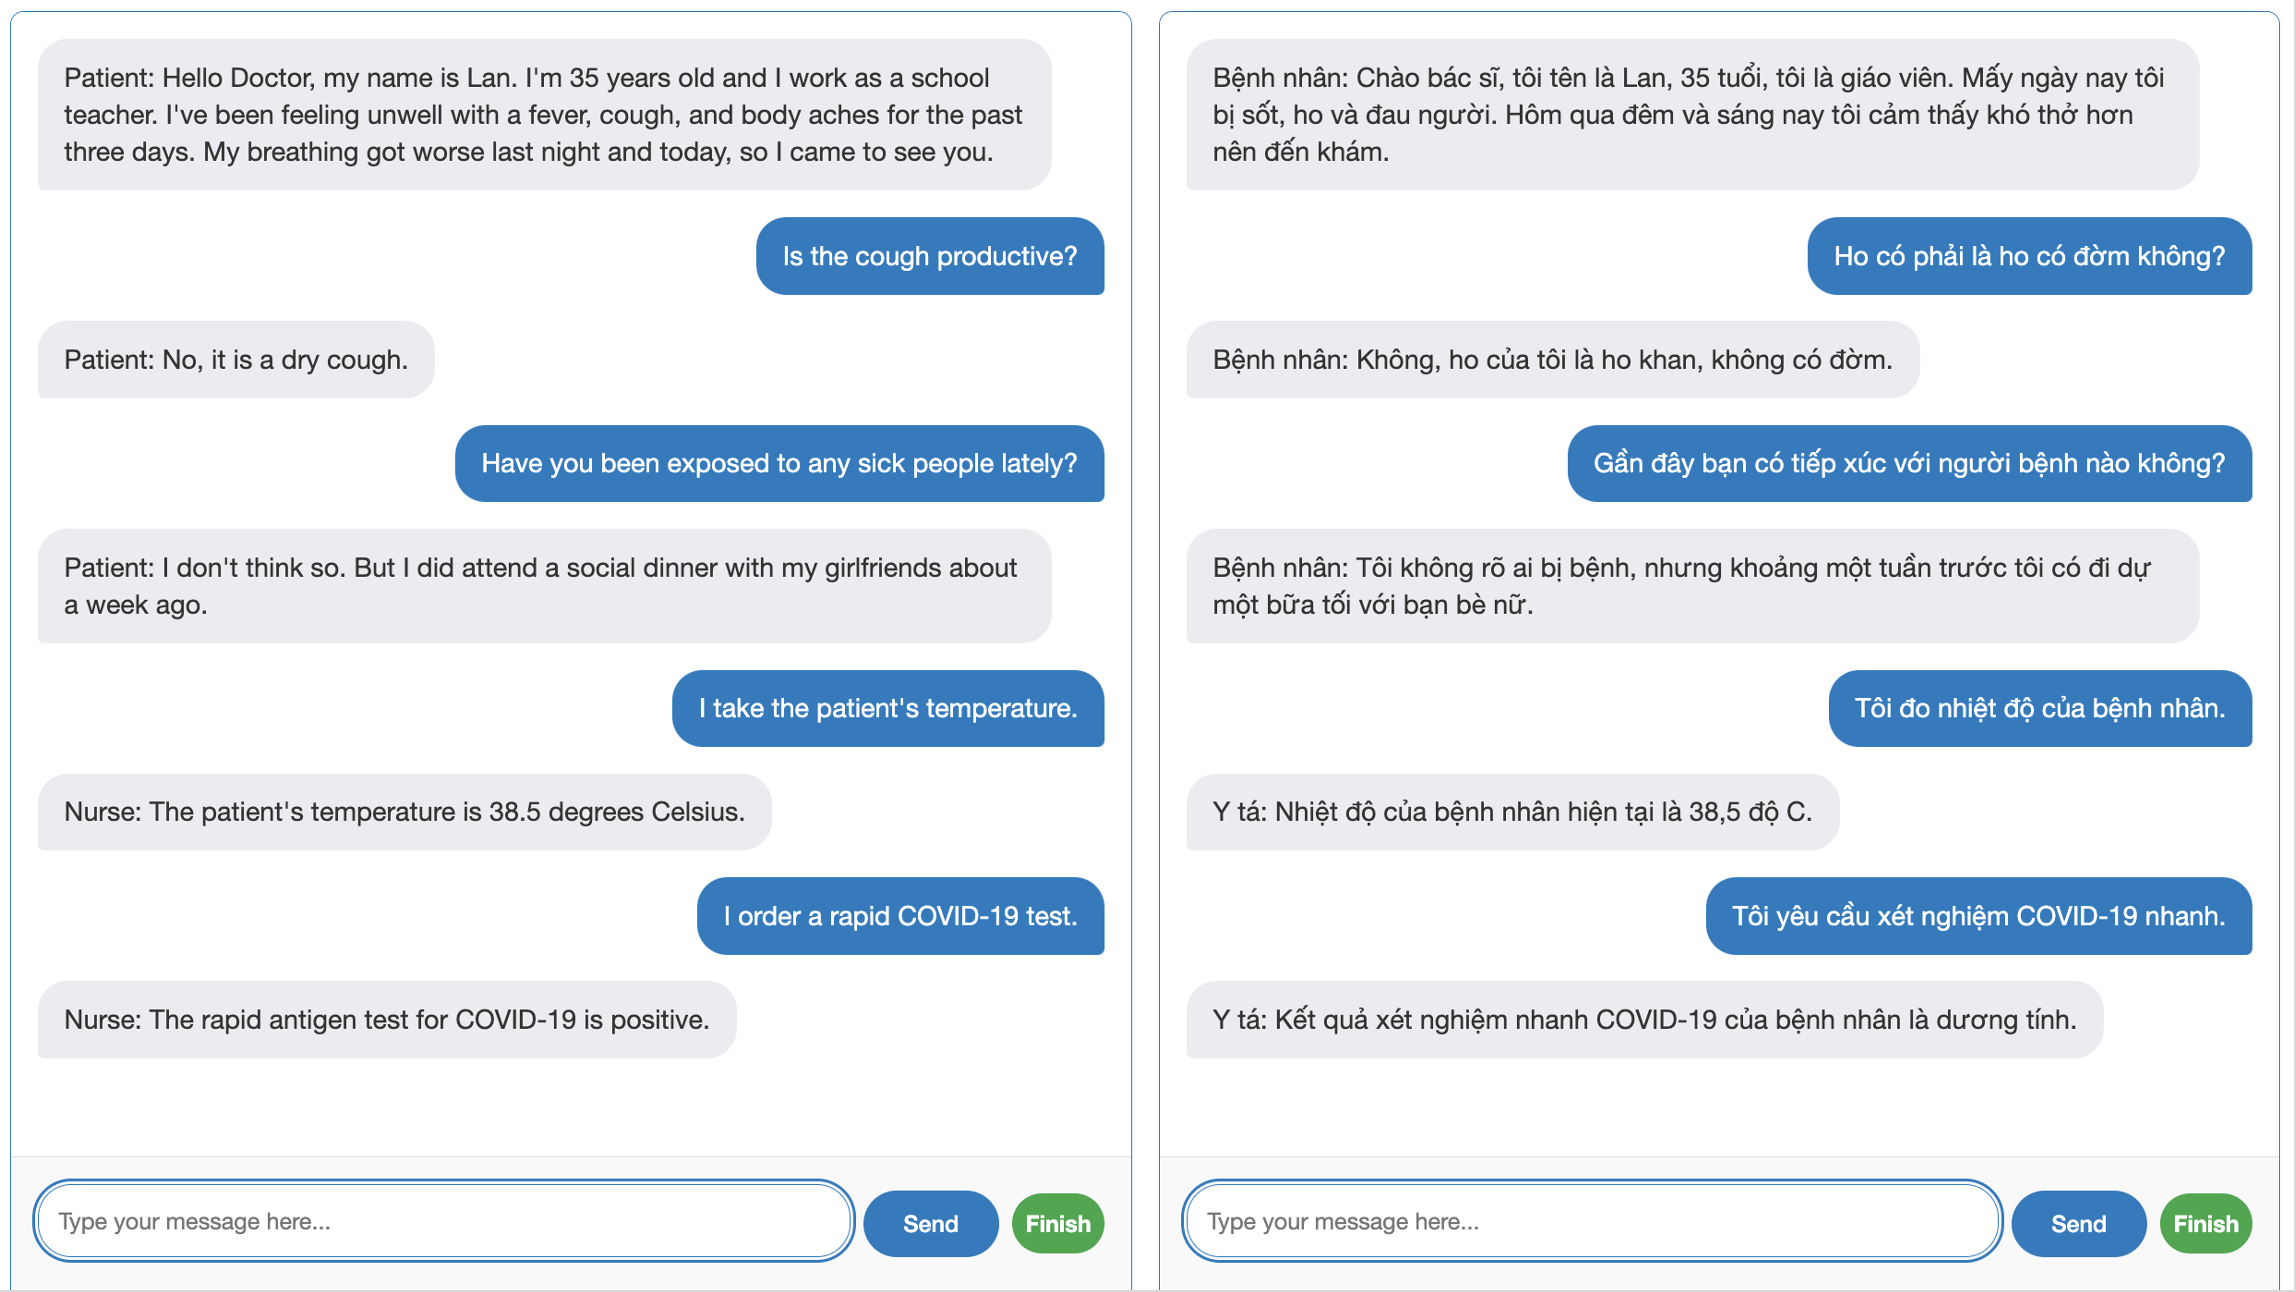
\includegraphics[width=\textwidth]{appendix/chatbot-screenshot.jpg}
  \caption{Screenshot of the LLM-based chatbot interface deployed through SurveyCTO. Left: English translation. Right: Original Vietnamese. The provider (blue bubbles) asks clinical questions and orders examinations; the LLM-simulated patient (grey bubbles) responds according to a pre-scripted clinical scenario. The interface runs on any smartphone or laptop browser.}
  \label{fig:chatbot}
\end{figure}

%% ————————————————————————————————
%% MATERIALS AND METHODS
%% ————————————————————————————————

\section{Materials and methods}

\subsection{Study design and participants}

In August 2025, we administered a web-based SurveyCTO survey (either by laptop or by mobile phone) that included LLM-based virtual patient ``chatbots'' preloaded with a pool of ten clinical cases (five general primary care conditions and five hepatitis-related) (\textbf{Table \ref{tab:cases}}). Each case scenario -- detailing the patient's socioeconomic background, chief complaint, medical history, clinical exam results, and potential responses to a set of ``checklist'' questions -- was scripted by expert clinicians supporting the research team. The OpenAI application programming interface (API; model gpt-4.1-nano) was prompted through the SurveyCTO software to perform according to these scenarios such that reasonable standardization was achieved across interactions. The scenarios developed for this study are available in the \textbf{Supporting Information}.

The research team first recruited and consented 9 physicians from a Provincial Hospital in Phu Tho, Vietnam, to a focus group for usability testing and UI/UX refinement. These providers received a live demonstration by the research team and were instructed to complete as many case scenarios as they found reasonable in a 45-minute period, followed by closed-ended (Likert scale) feedback questions on the realism of each case presentation. Two days later, the team conducted a structured group discussion to collect open-ended feedback, which was incorporated into the validation round.

For the validation sample, the research team contacted and consented 22 providers enrolled in the 2024-5 cohort of the StITCH hepatitis care training program, which co-designed and delivered a people-centered model of care for hepatitis B and C at the primary health care level in Vietnam. The validation group was given a Zoom orientation with no additional in-person support. These providers were assigned to complete six vignettes selected at random (three general cases and three hepatitis cases each). Afterwards, they completed a traditional multiple-choice knowledge test on hepatitis care, which included clinical knowledge questions based on the same five hepatitis scenarios. Although the total number of providers included in the validation sample was small, they completed 132 interactions containing 433 unique data points, allowing sufficient independent variation to assess the relationships between performance measures given that we do not engage in statistical hypothesis testing.

\subsection{Chatbot implementation}

The chatbot interface was built using the SurveyCTO platform's web-based survey tools with an LLM plugin \citep{geiecke2024conversations, surveycto2025llm}. Each clinical case was encoded as a structured system prompt (1,500--3,000 words) containing: the patient's demographic background and presenting complaint; a comprehensive medical and social history; pre-scripted responses to anticipated history-taking questions organized by clinical domain; clinical examination findings to be revealed when specific examinations were ordered; laboratory and imaging results for relevant tests; and the correct diagnosis with recommended treatment and counseling points. To maintain standardization, the system prompt instructed the model to report results as ``normal'' or ``unremarkable'' for tests not specified in the case scenario, and to stay in character as the patient throughout the interaction. The full set of case prompts is available in the \textbf{Supporting Information}.

The OpenAI model gpt-4.1-nano was selected after testing various model options for speed of response, cost-efficiency, and adequate performance in Vietnamese-language roleplay. The SurveyCTO plugin manages conversational state by appending each user message and model response to the conversation history, which is passed in full with each subsequent API call. Providers accessed the survey on their personal smartphones or laptops via a URL link. The chatbot responded in Vietnamese (selected by every provider) and maintained conversational context throughout each interaction. Providers could ask history-taking questions, order clinical examinations and laboratory tests, and provide a diagnosis and treatment plan, all through natural-language text input.

\subsection{Data extraction and coding}

Interaction transcripts were translated from Vietnamese to English using the Google Translate API and manually coded by the research team to determine whether each provider: (1) asked each of the pre-specified checklist history-taking questions, (2) ordered the recommended clinical examinations and laboratory tests, and (3) offered the correct diagnosis. The transcripts were also coded using the Anthropic Claude model (claude-haiku-4-5) with an identical rubric. The model was prompted to evaluate each transcript against all rubric items simultaneously: given the transcript, the provider's stated diagnosis, and their treatment plan, the model determined for each item whether the provider addressed it (scored 1 with a supporting quote from the transcript) or did not (scored 0). In a second pass, the model was additionally asked to report a confidence level between 0.0 and 1.0 for each item score, enabling receiver operating characteristic (ROC) analysis. To assess whether a separate translation step was necessary, we ran both the binary and confidence-scored LLM coding on the original Vietnamese transcripts as well as the English translations, using the same model and rubric. Using the human-coded and LLM-coded checklist items separately, a ``checklist score'' was calculated for each vignette response as the proportion of items completed.

\subsection{Outcomes}

For the focus group, primary outcomes were: (1) qualitative feedback on the LLM-based vignette survey obtained through the focus group discussion, and (2) quantitative ratings of scenario presentation realism. For the validation sample, the primary outcome was validation of the human-coded ``essential diagnostic checklist'' LLM vignette score via interaction-level correlations with expert clinician grading of the transcripts both in English and in the original Vietnamese. Our secondary outcomes were: (1) the reliability of the LLM-coded ``essential diagnostic checklist,'' assessed by correlation with ground truth from human coding; and (2) a comparison of LLM coding from translated English transcripts versus directly from the original Vietnamese transcripts.

\subsection{Statistical analysis}

For the focus group, the transcript was thematically analyzed by the research team to identify common themes for tool refinement. Provider perceptions of vignette realism were captured through structured survey questions rating overall realism, clinical presentation realism, and social/economic presentation realism. We calculated means and 95\% confidence intervals for each.

For the validation sample, agreement between manual and automated data extraction was assessed by calculating the proportion of agreement, true positives, false positives, true negatives, and false negatives based on the human coding as ground truth. The discriminative ability of the LLM coding was evaluated using receiver operating characteristic (ROC) analysis: for each item, the LLM's implied probability of positive classification (defined as the reported confidence when the binary score was 1, and 1 minus the confidence when the binary score was 0) was used as a continuous predictor against the human-coded gold standard, and the area under the ROC curve (AUROC) was computed. The two expert clinicians who developed the vignettes also scored provider performance on each transcript from 1--5 separately for history-taking, diagnosis accuracy, and management completeness (one using the Vietnamese original and one using the English translation). Agreement of the human grading with each of these measures was assessed through unadjusted ordinary least squares (OLS) regression. Clustering was not necessary in any case since we calculated results separately by scenario -- no provider repeated the same scenario twice. This study is reported following the Strengthening the Reporting of Observational Studies in Epidemiology (STROBE) guidelines for the observational validation design. A completed checklist is provided in the \textbf{Supporting Information}.

\subsection{Ethical approval}

All procedures were approved by the ethical review board of the Hanoi University of Public Health (025-375/DD-YTCC) and Mass General Brigham Institutional Review Board (Protocol Number 2023P003011). All participants provided written informed consent prior to participation.

%% ————————————————————————————————
%% RESULTS
%% ————————————————————————————————

\section{Results}

\subsection{Focus group}

Seven of the nine providers completed six cases within the allotted 45-minute focus group session, with average interaction time ranging from 3.4 to 9.2 minutes per case. All interactions were conducted in Vietnamese on smartphones. Across all conditions, respondents rated overall case realism positively, with an average of 3.78/5 (95\% CI: 3.65--3.90).

Qualitative feedback highlighted several notable strengths. Providers consistently emphasized the ease of use and user-friendliness of the LLM-based conversational vignettes: \textit{``Compared to other research tools, this one has a simpler interface and is easier to operate.''} Fast and contextually appropriate responses were the most frequently cited benefits (4 mentions), with providers noting that information provided was sufficient and meaningful for clinical decision-making: \textit{``The virtual patient's responses are relatively accurate, realistic, and easy to work with.''} Others commended its realism, including language localization and the ability to return to history-taking after laboratory results were delivered: \textit{``The language has been fully localized into Vietnamese and [is] very understandable''}; \textit{``It doesn't give us everything at once for us to guess. The more we ask, [\ldots] the more accurate the diagnosis will be.''} Another physician summarized: \textit{``Regarding the system's responses [\ldots], the level of realism is good. If we guide or structure our questions clearly, it will deliver as expected.''}

A few respondents noted minor issues. The most common limitation was that certain laboratory or imaging tests were not performed or had results omitted (4 mentions). \textit{``Some para-clinical tests weren't done, but when I asked a few related questions, [the responses] felt complete.''} Although the limited test results raised concerns regarding realism, this was an intentional design feature to ensure reasonable standardization of the virtual patients: tests deemed irrelevant for the case were prompted to have results reported as ``normal'' or ``unremarkable.'' The absence of non-verbal cues was also considered a barrier to realistic clinical interaction: \textit{``When we see patients in person, we can quickly evaluate whether there is an infectious syndrome. For asthma patients, just by observing their breathing we can tell how severe their respiratory distress is. But in a simulation, we are limited in the questions we can ask.''}

Respondents recommended several enhancements for future development. Suggestions included integrating visual elements such as laboratory images and video patient profiles, adding automatic performance feedback, and eventually transitioning from a web-based platform to an independent, offline smartphone application. One respondent also mentioned the potential benefit of including more complicated case scenarios to match clinical reality: \textit{``In real hospitals, most patients don't just have one disease -- they usually have multiple comorbidities.''} Overall, the focus group participants judged the LLM-based vignette survey to be both usable and realistic.

\subsection{Validation sample}

Twenty-two providers completed 132 interactions in the validation sample; two interactions were excluded due to incomplete transcript coding, leaving 130 for analysis (\textbf{Table \ref{tab:cases}}). The average interaction lasted 10.19 minutes (95\% CI: 9.03--11.35), excluding outliers lasting longer than one hour. The typical interaction resulted in the completion of 16.25\% of the essential diagnostic checklist items for that case scenario (95\% CI: 14.74--17.77). This low completion rate reflects the deliberately comprehensive nature of the checklists (30--55 case-specific items plus 19 common items per case; \textbf{Table \ref{tab:cases}}), which are designed to capture the full range of possible diagnostic actions rather than a minimum standard; similar checklist-based studies have reported comparable completion rates, as providers typically focus their history-taking on the most clinically relevant questions rather than exhaustively covering all possible items \citep{das2005which, daniels2024medical}. Based on the Vietnamese transcripts, the first clinical expert rated the average interaction 3.42 on a 1--5 scale (95\% CI: 3.24--3.59); based on the English transcripts, the other expert rated the average interaction 3.21 (95\% CI: 3.05--3.37). The two expert ratings agreed well, with some variation (Pearson's $\rho$ = 0.62, ordinary least squares [OLS] $r^{2}$ = 0.38). Compared with the human-coded score on the essential diagnostic checklist, the expert ratings had Pearson's $\rho$ = 0.55 and 0.60 for Vietnamese and English, respectively (\textbf{Figure \ref{fig:validation}}, Panels A and B). In regression, a 10 percentage point (p.p.)\ increase in the checklist completion corresponded with an approximate 0.64-point increase in the expert rating.

\begin{table}[htbp]
\centering
\caption{Clinical case scenarios and validation summary. Each provider completed six randomly assigned cases ($n$ = 130 interactions from 22 providers, excluding two with incomplete transcript coding). Items column shows total checklist items per case (case-specific plus 19 common items administered across all cases). Checklist completion and expert ratings are condition-level means.}
\label{tab:cases}
\begin{tabular}{clcccrrr}
\toprule
Case & Condition & Category & $N$ & Items & Checklist (\%) & Expert (VN) & Expert (EN) \\
\midrule
1 & Asthma & General & 14 & 62 & 12.1 & 3.07 & 3.71 \\
2 & Pneumonia & General & 14 & 49 & 23.3 & 3.79 & 3.36 \\
3 & Type 2 diabetes & General & 13 & 58 & 15.4 & 3.77 & 3.08 \\
4 & Pulmonary tuberculosis & General & 13 & 58 & 21.5 & 3.15 & 3.23 \\
5 & Hypertension & General & 11 & 56 & 16.7 & 3.45 & 3.09 \\
6 & Hepatitis B (chronic) & Hepatitis & 14 & 74 & 11.4 & 3.07 & 2.50 \\
7 & Hepatitis B (pregnancy) & Hepatitis & 12 & 62 & 13.2 & 3.42 & 3.17 \\
8 & Hepatitis B (vaccination) & Hepatitis & 13 & 58 & 15.5 & 3.46 & 3.15 \\
9 & Hepatitis C & Hepatitis & 14 & 64 & 16.9 & 3.50 & 3.29 \\
10 & HIV/antiretroviral therapy & Hepatitis & 12 & 63 & 16.5 & 3.50 & 3.50 \\
\midrule
 & \textit{Overall} & & 130 & & 16.3 & 3.42 & 3.21 \\
\bottomrule

\end{tabular}
\end{table}

The LLM-automated coding from translated English transcripts was moderately correlated with the human coding (Pearson's $\rho$ = 0.53; OLS $r^{2}$ = 0.28), with a 10 p.p.\ increase in the human-coded essential diagnostic checklist predicting a 5.9 p.p.\ increase in the LLM-coded checklist (\textbf{Figure \ref{fig:validation}}, Panel D). When the LLM coded directly from the original Vietnamese transcripts -- without a separate translation step -- performance was comparable (Pearson's $\rho$ = 0.51; OLS $r^{2}$ = 0.26; \textbf{Figure \ref{fig:validation}}, Panel C), suggesting that translation is not a binding constraint for multilingual deployment.

The discriminative ability of the LLM coding was assessed using ROC analysis, treating the human coding as the gold standard and the LLM's confidence-weighted probability as the continuous classifier (\textbf{Figure \ref{fig:agreement}}). The AUROC for English transcript coding was 0.87 and for Vietnamese transcript coding was 0.87, indicating good discriminative ability in both languages. The ROC curves for both languages were similar in shape, consistent with the finding that direct Vietnamese coding performs comparably to coding from English translations.

\begin{figure}[htbp]
  \centering
  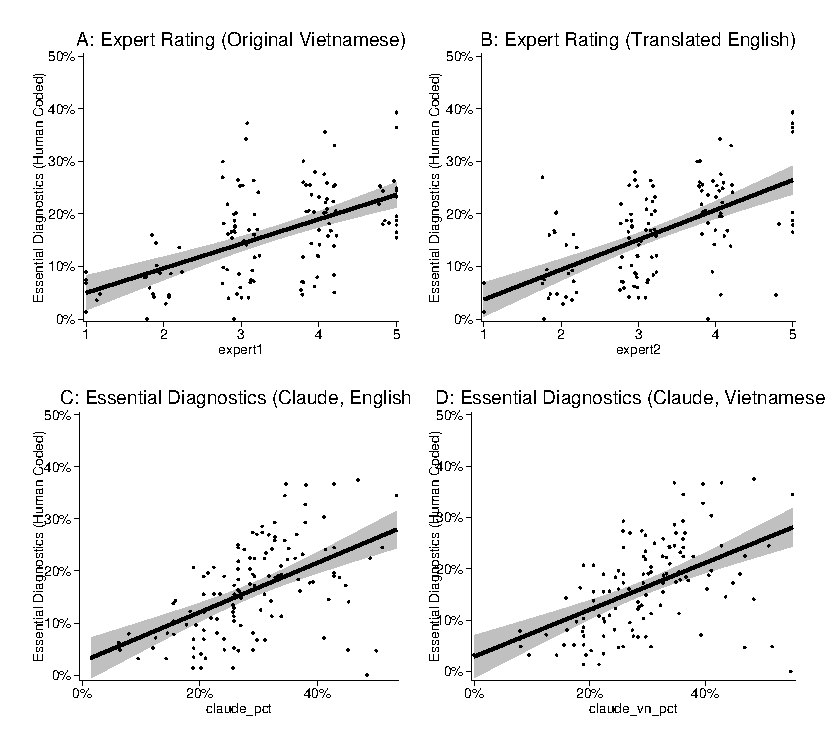
\includegraphics[width=\textwidth]{exhibits/F2.pdf}
  \caption{Validation of essential diagnostic checklist scores. Human-coded checklist completion (vertical axis) plotted against: Panel A: expert rating from original Vietnamese transcripts; Panel B: expert rating from translated English transcripts; Panel C: Claude-coded checklist directly from Vietnamese transcripts; Panel D: Claude-coded checklist from English transcripts. Each point is one provider--case interaction. Lines show OLS fit with 95\% confidence interval.}
  \label{fig:validation}
\end{figure}

\begin{figure}[htbp]
  \centering
  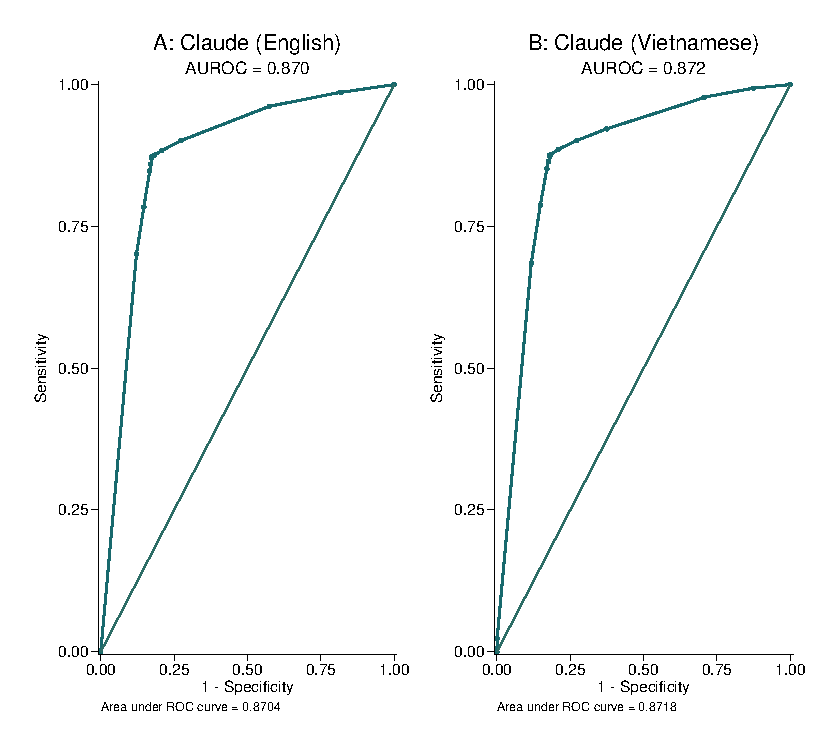
\includegraphics[width=\textwidth]{exhibits/F3.pdf}
  \caption{Receiver operating characteristic (ROC) curves for LLM coding of checklist items against human-coded gold standard. Panel A: coding from translated English transcripts. Panel B: coding directly from Vietnamese transcripts. The diagonal dashed line represents chance performance (AUROC = 0.5). AUROC values are shown in subtitles.}
  \label{fig:agreement}
\end{figure}

%% ————————————————————————————————
%% DISCUSSION
%% ————————————————————————————————

\section{Discussion}

Our results demonstrate that LLM-driven conversational vignettes produce competency measures that correlate well with expert evaluations of provider performance (Pearson's $\rho$ = 0.55--0.60). The method eliminates the need for in-person enumerators while preserving the open-ended interaction format that is the foundation of vignette validity \citep{das2005which}. The platform's practical utility is substantial: 132 clinical interactions were completed at a total chatbot cost of under USD 2, with no in-person support beyond a brief Zoom orientation -- a fraction of the cost of traditional in-person vignette surveys, which typically require two trained enumerators per interaction plus travel and per diem costs \citep{andrews2021quality}.

We found that the Anthropic Claude LLM was able to extract structured data from transcripts to our specifications, and that these data correlated moderately with human-coded ground truth (Pearson's $\rho$ = 0.53; OLS $r^{2}$ = 0.28). Notably, LLM coding performed comparably when applied directly to Vietnamese transcripts ($\rho$ = 0.51; $r^{2}$ = 0.26), without a separate translation step. This finding has practical significance: it suggests that multilingual deployment does not require an intermediate translation pipeline, reducing both cost and potential for translation-induced error. This pattern is consistent with recent benchmarks of LLM-based clinical scoring, where automated systems achieve moderate agreement with human evaluators but struggle with nuanced interpretation of free-text responses \citep{geathers2025benchmarking, kuling2026assessment}. While LLM-assisted translation and human data extraction was not excessively burdensome at this scale, further research on the reliability and cost of automated data extraction may streamline data encoding at larger scales. Automated data extraction also preserves complete data in the form of transcripts and could enable future refinement or modification of checklists to fit the research purpose, rather than pre-encoding the data structure. Future research might also assess more expensive models, such as modern ``reasoning'' models, or develop a multi-shot ``voting'' algorithm to overcome some of its variability.

Our approach extends the emerging literature on LLM-based virtual patients \citep{zeng2025embracing, cook2025virtual} in two important ways. First, whereas most existing applications target medical students in high-income educational settings, we demonstrate feasibility for health workforce assessment among practicing providers in a low- and middle-income country context. Second, we validate the resulting competency scores against independent expert clinician ratings, providing evidence that LLM-based vignettes measure meaningful dimensions of clinical competence. Third, we show that LLM-based data extraction performs comparably in Vietnamese and English, demonstrating feasibility for direct multilingual deployment without a separate translation pipeline. Future directions for tool refinement may include incorporating audio or video patient profiles to enhance realism through non-verbal cues.

The need for scalable competency measurement is acute. Evidence from sub-Saharan Africa \citep{daniels2024medical}, South and Southeast Asia \citep{das2022two, sassi2024impact, zhang2024quality, harrison2015patient}, and Vietnam specifically \citep{demombynes2016quality, zawahir2021standardised} demonstrates that delivered care quality remains low despite growing investments in medical education, and that progress has been slow. The most recent comprehensive assessment of primary care quality in Vietnam using clinical vignettes was conducted in 2015 \citep{demombynes2016quality}; the expense of replication has prevented a post-pandemic update. Tools like the one presented here could enable continuous, routine monitoring at a fraction of the cost of traditional approaches.

\subsection{Limitations}

This study has several limitations. First, the sample size was small (22 providers, 132 interactions), which limits the precision of our validation estimates and may not capture the full range of provider behavior. Second, the study was conducted in a single country (Vietnam) with a specific set of clinical conditions; generalizability to other settings, languages, and health systems requires further investigation. Third, while the LLM-automated coding of checklist items was moderately correlated with human coding ($\rho$ = 0.51--0.53), the ROC analysis indicates that the LLM's discriminative ability, though good (AUROC = 0.87), is imperfect, and classification errors could systematically bias competency estimates if used without human review. Fourth, we validated against human-coded checklists and expert ratings, but did not compare against direct clinical observation; the well-documented ``know-do gap'' means that vignette-based competency measures may not fully reflect actual practice \citep{ibnat2019three}. Fifth, the text-based interaction format inherently lacks non-verbal clinical cues (e.g., visual inspection, auscultation sounds), which may constrain the types of clinical reasoning that can be assessed. Sixth, LLM behavior may vary across model versions and over time, which could affect reproducibility; we report specific model versions to facilitate replication. Finally, the platform requires internet connectivity and smartphone access, which may limit deployment in the most resource-constrained settings.

\subsection{Conclusion}

This study demonstrates that LLM-driven conversational vignettes can produce a low-cost, flexible, and scalable platform for measuring health care provider competencies. The method eliminates the need for in-person enumerators while preserving the open-ended interaction format that is the foundation of vignette validity. The platform is open-source, built on widely used survey software, and designed for adaptation to a wide variety of clinical contexts and languages. As LLM capabilities continue to improve, both the chatbot interactions and the automated data extraction are likely to become more reliable, further reducing the cost and increasing the feasibility of routine competency measurement. With further validation across settings and languages, this method has the potential to support rapid, low-cost measurement of health care provider competencies in diverse health system contexts.

%% ————————————————————————————————
%% ACKNOWLEDGMENTS
%% ————————————————————————————————

\section*{Acknowledgments}

We acknowledge support in clinical vignette development, as well as transcript grading, from Dr.\ Marwatunnisa Al Mubarokah. We acknowledge additional support in vignette development and localization, as well as in leading the focus group and transcript grading, from Dr.\ Pham Thanh Thuy. We acknowledge the invaluable assistance, advice, and logistical coordination from Thu Huyen Nguyen and the rest of the staff at HAIVN. We acknowledge support in technical development of the survey plugin by Amrik Cooper and Mofya Phiri of Dobility, Inc.\ (SurveyCTO). We thank the participants in the focus group, management at Phu Tho Province General Hospital, and all respondents and StITCH program staff for their time, expertise, and feedback.

%% ————————————————————————————————
%% REFERENCES
%% ————————————————————————————————

\newpage
\bibliographystyle{unsrtnat}
\bibliography{sample}

%% ————————————————————————————————
%% REQUIRED PLOS SECTIONS
%% ————————————————————————————————

\newpage

\section*{Author contributions}

\noindent \textbf{Conceptualization:} BD, DD.
\textbf{Data curation:} BD, WSZ, HN.
\textbf{Formal analysis:} BD.
\textbf{Funding acquisition:} BD, DD.
\textbf{Investigation:} BD, WSZ, HN.
\textbf{Methodology:} BD, DD.
\textbf{Project administration:} BD, HN, DD.
\textbf{Resources:} DD.
\textbf{Software:} BD.
\textbf{Supervision:} BD, DD.
\textbf{Validation:} BD, WSZ.
\textbf{Visualization:} BD.
\textbf{Writing -- original draft:} BD.
\textbf{Writing -- review \& editing:} BD, WSZ, HN, DD.

\section*{Data availability statement}

All data and code needed to reproduce the analyses in this study -- including clinical case rubrics, interaction transcripts, human and LLM coding, expert ratings, and analytical scripts -- are publicly available at \url{https://github.com/bbdaniels/vn-llm-pilot}.

\section*{Competing interests}

The authors declare no competing interests.

\section*{Financial disclosure}

This work was supported by the Harvard University Asia Center, the Harvard University Rose Service Learning Fellowship program, the Harvard University Institute for Quantitative Social Science, and Gilead Sciences. The funders had no role in study design, data collection and analysis, decision to publish, or preparation of the manuscript.

\end{document}
